\chapter{Background}

%<Paragraph> Overview of background

This chapter provides a background of molecular computation techniques.  We explore nanotechnology and microbiology as a medium for computation and storage.  This begins with the foundations of nanotechnology, and continues with an example of encoding information with molecular matter.  Adleman's molecular computer for solving an instance of {\sc Hamiltonian Path} motivates the molecular operators and storage with DNA.

Finally, we provide an introduction to {\sc Satisfiability}.  This consists of development of the definition for {\sc Satisfiability} as a circuit.  We then view {\sc Satisfiability} as a language.  This provides a connection to other \textsf{NP-complete} problems through polynomial-time reductions.  We consider practical techniques for evaluating {\sc Satisfiability}.  This includes standards for input and output, along with an overview of {\sc Satisfiability} instance classification. 

\section{On nanotechnology and construction of molecules}

%		<Paragraph> Richard Feynman [introduces] nanotechnology
		
			Richard Feynman considered the possibility of construction of tiny machines from molecular interactions at the quantum scale.  Feynman founded the field of nanotechnology in his 1959 talk `There's Plenty of Room at the Bottom' \cite{feynman1959}.
			
%		<Paragraph> Applied nanotechnology [controls] materials
We are in an age of applied nanotechnology. Presently, we have the ability to control molecules and atoms through industrial processes. Examples of these processes include the manufacturing of graphene and DNA nanopores \cite{dnaTransistorIBMpressrelease}. Graphene consists of an arrangement of carbon atoms that provides desirable physical and electrical properties \cite{Stankovich_Dikin_Dommett_Kohlhaas_Zimney_Stach_Piner_Nguyen_Ruoff_2006}. DNA nanopores create a physical channel for threading DNA for read and write operations.  Diverse applications continue to take advantage of properties of nanotechnology.  Gene sequencing technologies provide an example of applied nanotechnology.  					
			%The work has driven the fields of molecular and quantum computation, VLSI circuit construction, and continues with innovative design and applications into many everyday processes.
		
%		<Paragraph> DNA substrate [builds] molecular definition
		
Smaller and cost effective DNA sequencers provide the ability to read the contents of a gene. Introduction of benchtop sequencers allows doctors to treat patients at their genome level from their office. Life Technologies and Oxford Nanopore offer gene sequencers based on solid-state semiconductor technology \cite{ionTorrent, oxfordNanopore}.	

\section{On microbiology and computation}

%	<Paragraph> Microbiology [studies] molecular life
	
	Microbiology studies properties of molecular interactions that form organic structures.  In this project, we explore techniques from applied genetics as a means for generalized computation.  Construction of a molecular computer requires transcription of data onto sequences of DNA or RNA.  Sequences of DNA and RNA define proteins that encode structural components.  As a computational medium, the encodings match configurations of a computation state. 
	
%	<Paragraph> Genetic alphabet [defines] life
		
	The genetic alphabet defines a universal medium for proteins.  Each of the base pairs (A, C, G, T, U) transcribes redundant encodings of amino acids.  Sequences of amino acids form structure as proteins.  Redundant encodings in the each amino acid permit syntax errors without a functional abnormality.  This redundant encoding structure permits mutation in the third base pair of each amino acid without consequence on the entire string.

%	<Paragraph> Complex molecules [contain] unique strings 
	
	Strings of base pairs encode information as oligonucleotides.  A \textit{oligonucleotide} is a short string of genetic information.  There are several configurations for DNA and RNA; these include $+$RNA, $-$RNA, $+$DNA, $-$DNA, $\pm$RNA, $\pm$DNA and +mRNA \cite{baltimore1971exp}.  The polarity of the DNA sequence denotes the direction of genetic information.  $+$DNA gets denoted by $5'$---$3'$ and $-$DNA gets denoted by $3'$---$5'$.  We focus on $+$DNA and $-$DNA as a substrate for encoding configurations for computational states.
	
%	<Paragraph> Each string [builds] structure from proteins
	Arbitrary encodings that represent mappings from variables to physical oligonucleotides may have undesirable structure and functionality.  Conventional techniques for DNA computing employ variable mappings from a library of oligonucleotides.  These strings avoid undesirable configurations, such as, self-complementary sequences that form hairpins \cite{dnaComputingModels2008}.  The sequence definition defines folding of the protein and the energy required to replicate. 
	
%	<Paragraph> Molecular definition [constructs] machine
Molecular computation defines sequences to represent a computational state.  Let us consider two techniques for representing information with oligonucleotides.  These allow us to encode integer mappings as either a fixed width integer sequence or as a binary vector of information.

Representation of an integer sequence requires a systematic mapping of an oligonucleotide entry with an integer counterpart.  A fixed width representation map independent sequences on a readable boundary.  Now we explore an example for encoding an integer sequence with a sequence of oligonucleotides.  A sample mapping is provided in Table \ref{integer2OligoTable}.

\begin{table}[htdp]
\caption{A mapping of the integers $[0,5]$ with arbitrary oligonucleotide definitions.}
\begin{center}
\begin{tabular}{|c|c|c|}
\hline
 \textbf{Integer} & \textbf{Oligonucleotide} & \textbf{Reverse-complement}\\ \hline
0 & $5'$TCTCCC$3'$ & $3'$AGAGGG$5'$ \\
1 & $5'$AAACCC$3'$ & $3'$TTTGGG$5'$ \\
2 & $5'$GGTAAA$3'$ & $3'$CCATTT$5'$ \\
3 & $5'$CCCTCC$3'$ & $3'$GGGAGG$5'$ \\
4 & $5'$CTTTTC$3'$ & $3'$GAAAAG$5'$ \\
5 & $5'$CCTTCC$3'$ & $3'$GGAAGG$5'$ \\ \hline
\end{tabular}
\end{center}
\label{integer2OligoTable}
\end{table}%

Suppose that we would like to encode the sequence of integers $S$ as an equivalent oligonucleotide representation $O_1$.

We have 
\[
S = [1, 3, 4, 3, 2, 0]
\]
and 
\[
O_1 = 5'\text{AAACCC}\mid \text{CCCTCC}\mid \text{CTTTTC}\mid \text{CCCTCC}\mid \text{GGTAAA}\mid \text{TCTCCC}3'.
\]
Recovering the sequence $S$ from $O_1$ can be done several ways.  Because the definition of the sequence exists, we may use the reverse complement to match sequences.  Another method splits the sequence $O_1$ on the encoding width.  In this case, the encoding width is six base pairs.  Gene sequencing tools permit reading the sequence and interpretation of the data with Table \ref{integer2OligoTable}.

Another technique for representing data as an oligonucleotide requires an assumption for state order.  This is done by encoding an $n$-dimensional vector.  We consider a binary vector, without loss of generality, encoding an $m$-ary vector is possible through construction of $m$ independent integer states.

Suppose that we would like to encode a bit vector $B$ as an equivalent oligonucleotide representation $O_2$.

We have 
\[
B = \langle 0100110 \rangle
\]
with the oligonucleotide definitions for 0 and 1 represented by the entries in Table \ref{integer2OligoTable}, we have
\[
O_2 = 5'\text{TCTCCC}\mid \text{AAACCC}\mid \text{TCTCCC}\mid \text{TCTCCC}\mid \text{AAACCC}\mid \text{AAACCC}\mid \text{TCTCCC}3'.
\]

%0 TCTCCC
%1 AAACCC

%	<Paragraph> Interactions of molecules [performs] computation
Molecular computing takes advantage of the inherent storage mechanism for solving problems with molecular interactions.  These interactions include matching and replication mechanics.  Although this setting describes and artificial construction for a machine, the natural encodings of organisms also share the mechanics that we exploit.  Interactions of molecules provide mechanics for generalized computation with oligonucleotides.
	
%	<Paragraph> Satisfiability [permits] universal computation
In the following chapters, we describe molecular algorithms for {\sc Satisfiability} and provide insight to construction of a generalized molecular computer.  Next we provide a toolbox for molecular computation.  The tools presented permit generalized computation with molecular biology techniques.  We apply the techniques from Leonard Adleman's molecular computer with an example of his first experiment.

\section{Adleman's molecular toolbox for solving {\sc Hamitonian Path}}
	
%	<Paragraph> Leonard Adleman [performs] first molecular computation 
Leonard Adleman performed the first molecular computation in 1994 with recombinant DNA in a manual laboratory setting \cite{Adleman:1994:MCS:189441.189442}.  This experiment solved a six vertex instance of {\sc Hamitonian Path}, a \textsf{NP-complete} problem.  In this section, we describe the techniques applied in this experiment. We provide  definitions of Adleman's molecular toolbox from an example of the original problem instance.  This includes the molecular operations: append, extract, mix, split and purify construct.
%	<Paragraph> Molecular computation [encodes] information from graph with DNA

Each vertex gets assigned an independent oligonucleotide as we have done in Table \ref{integer2OligoTable}.  Possible solutions get stored in a test tube $T$.  $T$ begins as an empty tube.  We introduce equimolar portions of each string as a starting configuration with the \textit{mix} operation. 
\begin{definition}
\textit{Mix}\\
$ T \leftarrow \text{mix}( T_1, T_2)$ --- combines two test tubes of information.  The output consists of a single set $T = T_1 \cup T_2$.
\end{definition}

A small initial set may be amplified with \textit{polymerase chain reaction} (PCR).  PCR thermocycles the contents of the tube to replicate the contents. Possible paths get randomly generated by introducing the vertex representation to the contents.  We create this representation elongating the initial vertex with a fixed path length.

\textit{Append} attaches a string to each string contained in a test tube.  \textit{Split} portions a tube into multiple portions.  We will use split-mix synthesis as a technique for generation of combinatorial space in Chapter 3.
%A possible path is created by randomly appending sequences to create a uniform statistical distribution of all paths.  

\begin{definition}
\textit{Append}\\
$T' \leftarrow \text{append}( T, a)$ --- the concatenation of $a$ with each element in $T$.  
\end{definition}

\begin{definition}
\textit{Split}\\
$[T', T''] \leftarrow \text{split}( T)$ --- distributes $T$ into two tubes.  Each of the resulting tubes, $T'$ and $T''$,  contain the same representative elements of $T$.
\end{definition}

From the tube $T$, we keep paths that begin with $V_{in}$ and end with $V_{out}$.  This ensures that the initial and terminal conditions for the graph get satisified.  Extracting only strings from $T$ that match these conditions reduces the number of potential strings.

\begin{definition}
\textit{Extract}\\
$ T' \leftarrow \text{extract}( T, a, x)$ --- separates all strings from $T$ containing the literal $a$ at position $x$.  The output consists of a set $T'$ of those strings containing $a$ at position $x$.
\end{definition}

The tube $T$ consists of possible encodings that have the correct starting and ending vertices. We select only strings with length $n$ to ensure that all vertices get traversed.  This can be performed with \textit{gel electrophoresis}, a technique for sorting molecules by mass.

Next, we ensure that each vertex occurs exactly once.  This gets accomplished by extracting possible vertices.  If a vertex occurs multiple times in a path, then the string representation gets discarded.

Finally, we check $T$ with \textit{detect} to determine if any valid paths remain.  If valid paths exist, then each string may be read for the path assignment.

\begin{definition}
\textit{Detect}\\
$ \text{detect}( T)$ --- determine if any encodings are present in $T$.  The output consists of $true$ or $false$, for $T \neq \emptyset$ or $T = \emptyset$ respectively.
\end{definition}

\subsection{Additional molecular operators}

In the following chapters, we will use the molecular operators for construction of molecular {\sc Satisfiability} solvers.  The Distribution algorithm, introduced in Chapter 4, requires the \textit{splice} operation.
\begin{definition}
\textit{Splice}\\
$[a_1, a_2] \leftarrow \text{splice}(a, b)$ --- cuts a string $a$ with a subsequence $b$ into two pieces by a restriction enzyme.  These two pieces are $a_1$ and $a_2$.
\end{definition}

In the implementation of a simulation environment, we avoid redundant string representations with the \textit{purify} operation.  This is a synthetic version of PCR.  Purify balances the space representation of molecules with a uniform distribution.
\begin{definition}
\textit{Purify}\\
$T' \leftarrow \text{purify}(T)$ --- provides a uniform distribution from the contents of $T$ as $T'$.
\end{definition}

%	<Paragraph> Execution [solves] NP-complete problem instance	
%	<Paragraph> Encoding [requires] permutations of space	
%	<Paragraph> Subsequent molecular algorithms [constrain] required space

%\begin{definition}
%$[a_1, a_2] \leftarrow \text{splice}(a, b)$ --- is defined as cutting a string $a$ with a subsequence $b$ into two pieces by a restriction enzyme.  These two pieces are $a_1$ and $a_2$.
%\end{definition}
	
\section{Definition of {\sc Satisfiability}}

%	<Paragraph> Introduce and motivate {\sc Satisfiability}
	
{\sc Satisfiability} is a canonical \textsf{NP-complete} language.  Each {\sc Satisfiability} instance efficiently encodes a set of conditions to satisfy.  Because {\sc Satisfiability} is \textsf{NP-complete}, it can be reduced to any \textsf{NP-complete} language.

%	<Paragraph>	Define {\sc Satisfiability} with circuit 

Evaluation of a {\sc Satisfiability} instance requires validating the input with the instance definition.  We introduce {\sc Satisfiability} evaluation with a circuit.  Let us consider a three-layered circuit for {\sc Satisfiability}.  This circuit consists of $n$ inverters, $m$ \textbf{OR} gates, and one \textbf{AND} gate with $m$-fan-in.  This circuit behaves according to the internal wiring of the input expression $\phi$. Figure \ref{blackBoxSat} contains a schematic for {\sc Satisfiability}.	
%	<Figure>	Circuit description
\begin{figure}[htbp]
\begin{center}

	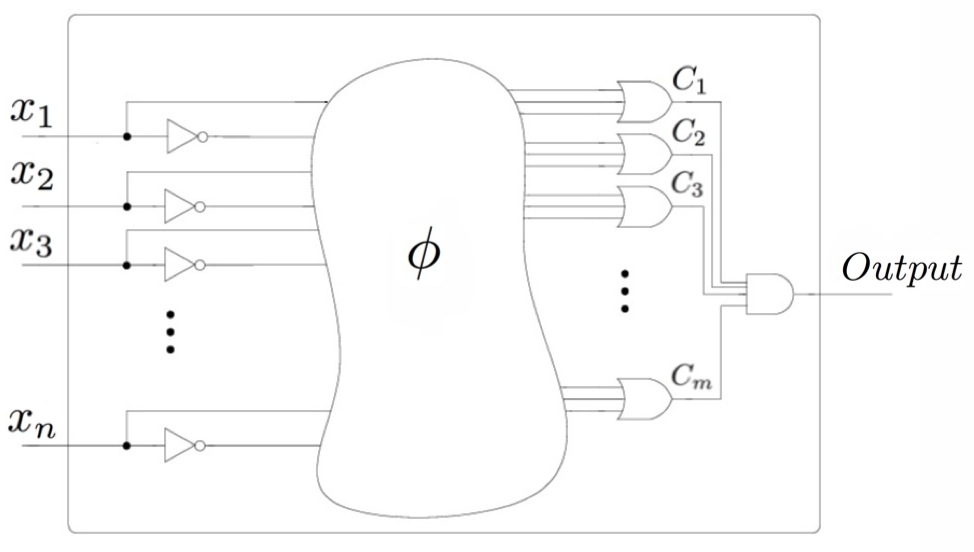
\includegraphics[width=0.9\textwidth]{figures/circuitLabeled.jpg}

\caption{A circuit describing {\sc Satisfiability}.}
\label{blackBoxSat}
\end{center}
\end{figure}
	
\FloatBarrier

%	<Paragraph> Provide complexity of {\sc Satisfiability}
The realization of {\sc Satisfiability} as a circuit shows two insights of the problem.  {\sc Satisfiability} can be implemented with logic components proportional to the problem size, and the worst case verification consists of enumerating all possible switch configurations.  {\sc Satisfiability} as a language demonstrates that it is equivalent to all other \textsf{NP-complete} languages.

Cook and Levin independently introduced the canonical instance of a \textsf{NP-complete} language {\sc Satisfiability}\cite{Cook:1971:CTP:800157.805047, levin1973}.  A \textsf{NP-complete} language is one that is in \textsf{NP} and \textsf{NP-hard}.  A \textsf{NP-hard} language is at least as hard as any problem in \textsf{NP}.

{\sc Satisfiability} may be formally defined as the language
\[
\text{\sc Satisfiability} = \{ \langle \phi \rangle \mid \phi \text{ is a satisfiable Boolean formula}\} \cite{sipser06}.
\]	
	
%	<Paragraph> Motivate practical input and classifying metrics 

The next section considers standards adopted for {\sc Satisfiability}.  This allows practitioners to apply {\sc Satisfiability} in various settings.
	
\section{Evaluating {\sc Satisfiability}}

%	<Paragraph> Overview of evaluation
	
	In this section, we consider standards for {\sc Satisfiability} instances.  This includes DIMACS CNF input and {\sc Sat} Competition output.  
	
	Next, we consider classification of {\sc Satisfiability} instances.  These include randomly generated, crafted and industrial problem instances.  Following, we examine metrics for classifying {\sc Satisfiability} instances.

	\subsection{Input and output}
	
%		<Paragraph> {\sc Satisfiability} standards [provide] common interface
	
  Conforming to standards allows datasets and common interfaces to be shared.  The input and output standards for {\sc Satisfiability} allow common benchmarks for {\sc Sat} solvers.  {\sc Sat} solvers demonstrate state-of-the-art techniques. Each year a competition showcases techniques for evaluating {\sc Satisfiability}.  We conform to the standards of the {\sc Sat} Competition \url{http://www.satcompetition.org/}.
	
		\subsubsection{Input}
		
%			<Paragraph> DIMACS CNF [provides] standard benchmark instances
DIMACS CNF provides standard input for {\sc Satisfiability} \cite{dimacsFormat}.  This format consists of {\sc Satisfiability} encoded in conjunctive normal form (CNF).  The format is user readable with a natural encoding for {\sc Satisfiability}.  We provide an example of this encoding in Section \ref{inputSection}.
		
		\subsubsection{Output}
		
%			<Paragraph> Sat Competition output [provides] standard output
{\sc Sat} Competition output \cite{satcompetition} provides a concise result for the state of a {\sc Satisfiability} instance.  The output consists of the known configuration and provides a valuation if the instance is satisfiable.  The output streams to standard output.  We provide an example along with a custom interface in Section \ref{outputSection}.
	
	\subsection{Metrics for classifying {\sc Satisfiability}}

%		<Paragraph> Describe metrics
{\sc Sat}-phase-transition and {\sc Sat}-backbones are two classifying metrics for {\sc Satisfiability}.  These metrics may be used to classify {\sc Satisfiability} expressions.  We will use these metrics in the next section for defining a sweep of random $k$-{\sc Sat} instances.
		
%		<Paragraph> {\sc Sat} phase transition

The {\sc Sat}-phase-transition is a region where both satisfiable and unsatisfiable instances may occur.  The ratio of clauses to variables $\alpha = m/n$ provide a classification for $k$-\textsf{CNF} formula \cite{Doherty08thehandbook,Gent94thesat}.
		
%		<Paragraph> {\sc Sat} backbones

{\sc Sat}-backbones are the variable assignments present in all of the satisfying assignments to a {\sc Satisfiability} expression \cite{Zhang2001}.  This is a set of variables that occur in all satisfiable valuations for an input expression.  

	\subsection{{\sc Satisfiability} instances}
		
%		<Paragraph> Various methods for [constructing] {\sc Satisfiability} instances
There are several methods for constructing {\sc Satisfiability} instances.  We consider techniques for constructing instances based on random assignment, crafted and real applications from industry.  The instance type demonstrate properties of {\sc Satisfiability} and provide heuristics for certain input.
	
%		<Paragraph> {\sc Satisfiability} instance [generated] from random assignment
A random $k$-{\sc Sat} expression consists of $m$ clauses with $k$ literals per-clause from  $n$ variables \cite{wilsonKsat}. Variable assignments get distributed with probability $Prob\left(\frac{1}{n}\right)$.  The positive or negative variable polarity get assigned with a probability $Prob\left(\frac{1}{2}\right)$.

%Random $k$-{\sc Sat} are generated with \texttt{ksat.c} \cite{wilsonKsat}.  A hash of the clause representation ensures that all clauses are independent \cite{wilsonKsat}.

%During generation of these formulas a hash is implemented to ensure that the random assignments ensure independent clauses and non-redundant variable assignments.  
		
%		<Paragraph> {\sc Satisfiability} instance [constructed] as hard assignment

Crafted instances provide difficult benchmark cases.  These instances can be converted from other \textsf{NP-complete} problems.  This category also includes games and graph theoretic problems represented as {\sc Satisfiability}. 
		
		
%		<Paragraph> {\sc Satisfiability} instance [applied] from real world problems

Industrial processes apply {\sc Satisfiability} in many real world problems.  This includes circuit layout, planning, logistics, circuit fault testing and many other industrial \textsf{NP-complete} problems.  Applications for industrial {\sc Sat} will often apply heuristics and approximation techniques to relax the problem.  This allows approximate solutions to be computed in an efficient amount of time.
		